\documentclass[journal]{IEEEtran}
\usepackage{tikz}
\usetikzlibrary{shapes,arrows.meta,positioning,fit,backgrounds,calc}
\usepackage{amsmath,amssymb}

\begin{document}

\begin{figure*}[!t]
\centering
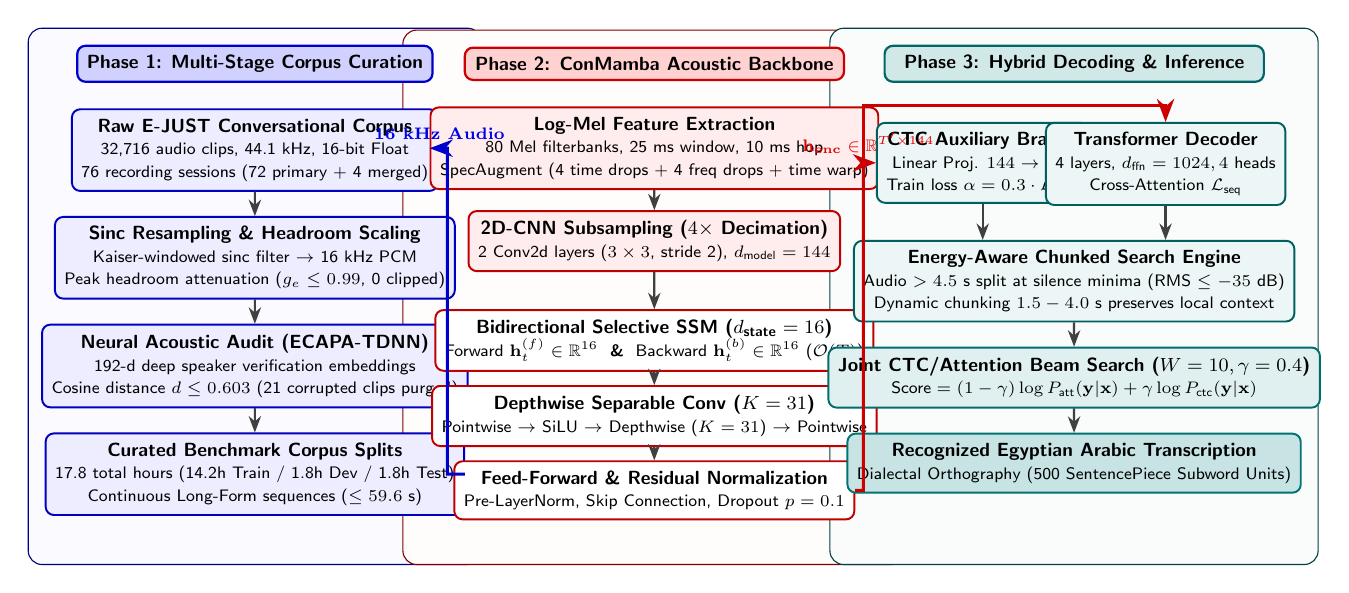
\begin{tikzpicture}[
    scale=0.86, every node/.style={transform shape},
    font=\sffamily\footnotesize,
    box/.style={rectangle, draw=#1!75!black, fill=#1!7, line width=0.7pt, rounded corners=3pt, align=center, inner sep=4pt},
    header/.style={rectangle, fill=#1!18, draw=#1!80!black, line width=0.8pt, rounded corners=3pt, font=\sffamily\bfseries\footnotesize, align=center, inner sep=4pt},
    blockframe/.style={rectangle, draw=#1!80!black, fill=#1!3, dashed, line width=0.8pt, rounded corners=4pt},
    arrow/.style={-{Stealth[scale=0.9]}, line width=0.8pt, draw=black!75},
    interarrow/.style={-{Stealth[scale=1.05]}, line width=1.1pt, draw=#1!80!black}
]

% =========================================================================
% COLUMN 1: PHASE 1 - ACOUSTIC CURATION PIPELINE
% =========================================================================
\node[header=blue, minimum width=5.2cm] (h1) at (0, 0) {Phase 1: Multi-Stage Corpus Curation};

\node[box=blue, below=0.38cm of h1, minimum width=5.0cm] (p1_raw) {
    \textbf{Raw E-JUST Conversational Corpus}\\
    \scriptsize 32,716 audio clips, 44.1 kHz, 16-bit Float\\
    \scriptsize 76 recording sessions (72 primary + 4 merged)
};

\node[box=blue, below=0.36cm of p1_raw, minimum width=5.0cm] (p1_resamp) {
    \textbf{Sinc Resampling \& Headroom Scaling}\\
    \scriptsize Kaiser-windowed sinc filter $\to$ 16 kHz PCM\\
    \scriptsize Peak headroom attenuation ($g_e \le 0.99$, 0 clipped)
};

\node[box=blue, below=0.36cm of p1_resamp, minimum width=5.0cm] (p1_ecapa) {
    \textbf{Neural Acoustic Audit (ECAPA-TDNN)}\\
    \scriptsize 192-d deep speaker verification embeddings\\
    \scriptsize Cosine distance $d \le 0.603$ (21 corrupted clips purged)
};

\node[box=blue, below=0.36cm of p1_ecapa, minimum width=5.0cm] (p1_splits) {
    \textbf{Curated Benchmark Corpus Splits}\\
    \scriptsize 17.8 total hours (14.2h Train / 1.8h Dev / 1.8h Test)\\
    \scriptsize Continuous Long-Form sequences ($\le 59.6$~s)
};

\draw[arrow] (p1_raw) -- (p1_resamp);
\draw[arrow] (p1_resamp) -- (p1_ecapa);
\draw[arrow] (p1_ecapa) -- (p1_splits);

% =========================================================================
% COLUMN 2: PHASE 2 - CONMAMBA ACOUSTIC BACKBONE
% =========================================================================
\node[header=red, minimum width=5.6cm] (h2) at (5.9, 0) {Phase 2: ConMamba Acoustic Backbone};

\node[box=red, below=0.38cm of h2, minimum width=5.4cm] (p2_fbank) {
    \textbf{Log-Mel Feature Extraction}\\
    \scriptsize 80 Mel filterbanks, 25 ms window, 10 ms hop\\
    \scriptsize SpecAugment (4 time drops + 4 freq drops + time warp)
};

\node[box=red, below=0.30cm of p2_fbank, minimum width=5.4cm] (p2_conv2d) {
    \textbf{2D-CNN Subsampling ($4\times$ Decimation)}\\
    \scriptsize 2 Conv2d layers ($3\times 3$, stride 2), $d_{\text{model}} = 144$
};

% ConMamba Stacked Blocks (Internal Layers)
\node[box=red, fill=white, below=0.55cm of p2_conv2d, minimum width=5.0cm] (p2_ssm) {
    \textbf{Bidirectional Selective SSM ($d_{\text{state}}=16$)}\\
    \scriptsize Forward $\mathbf{h}_t^{(f)} \in \mathbb{R}^{16}$ \ \textbf{\&}\ \ Backward $\mathbf{h}_t^{(b)} \in \mathbb{R}^{16}$ ($\mathcal{O}(T)$)
};

\node[box=red, fill=white, below=0.20cm of p2_ssm, minimum width=5.0cm] (p2_conv) {
    \textbf{Depthwise Separable Conv ($K=31$)}\\
    \scriptsize Pointwise $\to$ SiLU $\to$ Depthwise ($K=31$) $\to$ Pointwise
};

\node[box=red, fill=white, below=0.20cm of p2_conv, minimum width=5.0cm] (p2_res) {
    \textbf{Feed-Forward \& Residual Normalization}\\
    \scriptsize Pre-LayerNorm, Skip Connection, Dropout $p=0.1$
};

\draw[arrow] (p2_fbank) -- (p2_conv2d);
\draw[arrow] (p2_conv2d) -- (p2_ssm);
\draw[arrow] (p2_ssm) -- (p2_conv);
\draw[arrow] (p2_conv) -- (p2_res);

% Enclosing frame around ConMamba layers
\begin{scope}[on background layer]
    \node[blockframe=red, fit=(p2_ssm)(p2_res), inner sep=5pt,
          label={[red!85!black, font=\sffamily\bfseries\scriptsize]above:Stacked ConMamba Blocks ($\times 12$, 12.1M Params)}] (p2_blockframe) {};
\end{scope}

% Inter-phase arrow 1 -> 2 (Clean Gutter Routing)
\coordinate (g1) at ($(p1_splits.east)!0.5!(p2_fbank.west |- p1_splits.east)$);
\draw[interarrow=blue] (p1_splits.east) -- (g1) -- (g1 |- p2_fbank.west) -- (p2_fbank.west)
    node[pos=0.45, above, font=\scriptsize\bfseries, text=blue!90!black] {16 kHz Audio};

% =========================================================================
% COLUMN 3: PHASE 3 - HYBRID CTC/ATTENTION DECODING
% =========================================================================
\node[header=teal, minimum width=5.6cm] (h3) at (12.1, 0) {Phase 3: Hybrid Decoding \& Inference};

% Parallel Branches: CTC Branch on Left, Transformer Decoder on Right
\node[box=teal, below=0.58cm of h3.south -| {$(h3.center)+(-1.35,0)$}, minimum width=2.55cm] (p3_ctc) {
    \textbf{CTC Auxiliary Branch}\\
    \scriptsize Linear Proj. $144 \to 500$\\
    \scriptsize Train loss $\alpha = 0.3 \cdot \mathcal{L}_{\text{CTC}}$
};

\node[box=teal, below=0.58cm of h3.south -| {$(h3.center)+(1.35,0)$}, minimum width=2.65cm] (p3_dec) {
    \textbf{Transformer Decoder}\\
    \scriptsize 4 layers, $d_{\text{ffn}}=1024, 4\text{ heads}$\\
    \scriptsize Cross-Attention $\mathcal{L}_{\text{seq}}$
};

% Energy Chunking Engine below both branches
\node[box=teal, below=0.52cm of $(p3_ctc.south)!0.5!(p3_dec.south)$, minimum width=5.4cm] (p3_chunk) {
    \textbf{Energy-Aware Chunked Search Engine}\\
    \scriptsize Audio $>4.5$~s split at silence minima (RMS $\le -35$~dB)\\
    \scriptsize Dynamic chunking $1.5-4.0$~s preserves local context
};

% Joint Beam Search
\node[box=teal, fill=teal!12, draw=teal!85!black, below=0.36cm of p3_chunk, minimum width=5.4cm] (p3_beam) {
    \textbf{Joint CTC/Attention Beam Search ($W=10, \gamma=0.4$)}\\
    \scriptsize $\text{Score} = (1-\gamma)\log P_{\text{att}}(\mathbf{y}|\mathbf{x}) + \gamma \log P_{\text{ctc}}(\mathbf{y}|\mathbf{x})$
};

% Final Output
\node[box=teal, fill=teal!22, draw=teal!90!black, below=0.36cm of p3_beam, minimum width=5.4cm] (p3_out) {
    \textbf{Recognized Egyptian Arabic Transcription}\\
    \scriptsize Dialectal Orthography (500 SentencePiece Subword Units)
};

% Column 3 Internal Arrows
\draw[arrow] (p3_ctc.south) -- ++(0,-0.20) -| ($(p3_chunk.north)+(-1.35,0)$);
\draw[arrow] (p3_dec.south) -- ++(0,-0.20) -| ($(p3_chunk.north)+(1.35,0)$);
\draw[arrow] (p3_chunk) -- (p3_beam);
\draw[arrow] (p3_beam) -- (p3_out);

% Inter-phase arrow 2 -> 3
\coordinate (g2) at ($(p2_res.east)!0.4!(p3_ctc.west |- p2_res.east)$);
\draw[interarrow=red] (p2_res.east) -- (g2) -- (g2 |- p3_ctc.west) -- (p3_ctc.west)
    node[pos=0.4, above, font=\scriptsize\bfseries, text=red!90!black] {$\mathbf{h}_{\text{enc}} \in \mathbb{R}^{T' \times 144}$};

% Clean route to Transformer Decoder
\coordinate (split3) at ($(p3_ctc.north)!0.5!(p3_dec.north)+(0,0.24)$);
\draw[interarrow=red] (g2 |- p3_ctc.west) -- (g2 |- split3) -- (split3) -| (p3_dec.north);

% =========================================================================
% BACKGROUND CONTAINERS (EQUALIZED HEIGHT)
% =========================================================================
% Find common bottom anchor
\coordinate (common_bottom) at (0, -7.15);

\begin{scope}[on background layer]
    \node[draw=blue!50!black, fill=blue!2, rounded corners=5pt, fit=(h1)(p1_raw)(p1_splits)(h1 |- common_bottom), inner sep=6pt] (c1) {};
    \node[draw=red!50!black, fill=red!1, rounded corners=5pt, fit=(h2)(p2_fbank)(p2_blockframe)(h2 |- common_bottom), inner sep=6pt] (c2) {};
    \node[draw=teal!50!black, fill=teal!2, rounded corners=5pt, fit=(h3)(p3_ctc)(p3_dec)(p3_out)(h3 |- common_bottom), inner sep=6pt] (c3) {};
\end{scope}

\path let \p1 = (c1.south), \p2 = (c2.south), \p3 = (c3.south),
          \p4 = (c1.north), \p5 = (c2.north), \p6 = (c3.north) in
    \pgfextra{
        \typeout{COORD_REPORT: c1_north=\y4, c1_south=\y1}
        \typeout{COORD_REPORT: c2_north=\y5, c2_south=\y2}
        \typeout{COORD_REPORT: c3_north=\y6, c3_south=\y3}
    };

\end{tikzpicture}
\caption{System overview of the proposed empirical framework for dialectal Egyptian Arabic ASR. Phase 1 demonstrates the multi-stage acoustic curation pipeline on the EJUST corpus, resolving resampling-induced digital clipping via per-episode headroom attenuation ($g_e \le 0.99$), removing speaker outliers via ECAPA-TDNN neural embeddings, and building paired short-form and continuous long-form benchmarks ($<60$~s). Phase 2 depicts the hybrid acoustic backbone combining 2D-CNN subsampling ($4\times$), 12 stacked bidirectional ConMamba encoder blocks (with forward/backward selective SSMs and wide depthwise separable convolutions $K=31$), and LayerNorm residuals. Phase 3 illustrates the hybrid CTC/attention decoding topology, coupling a frame-level CTC projection ($\alpha=0.3$) with a 4-layer Transformer cross-attention decoder and energy-aware chunked beam search ($W=10, \gamma=0.4$) for robust long-form transcription over a 500-unit SentencePiece vocabulary.}
\label{fig:framework_overview}
\end{figure*}

\end{document}
